\section{Durchführung}
\label{sec:Durchführung}

Der Versuch wird nach \autoref{fig:aufbauOptik} aufgebaut.
\begin{figure}[H]
    \centering
    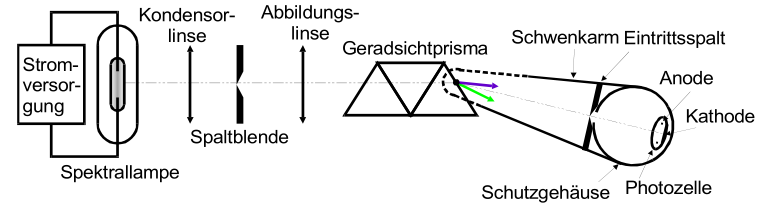
\includegraphics[width = 0.75\textwidth]{data/optischerTeil.png}
    \caption{Schematischer Aufbau des Versuches \cite{Anleitung500}.}
    \label{fig:aufbauOptik}
\end{figure}
Durch den Strahlengang, den das Licht durchzulaufen hat, wird es gebündelt und durch das Geradsichtprisma in verschiedene Wellenlängen aufgespaltet, sodass
die Photozelle mit monochromatischem Licht bestrahlt wird. Der prinzipielle Aufbau der Photozelle, der Teil des Versuchaufbaues, in dem der eigentliche Photoeffekt
stattfindet, ist in \autoref{fig:photozell} abgebildet.
\begin{figure}[H]
    \centering
    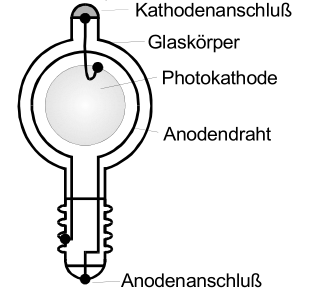
\includegraphics[width = 0.75\textwidth]{data/photozelle.png}
    \caption{Schematische Darstellung der in dem Versuch verwendeten Photozelle \cite{Anleitung500}.}
    \label{fig:photozell}
\end{figure}
